\documentclass{standalone}
\usepackage{tikz}
\usetikzlibrary{patterns, positioning}
\usepackage[sfdefault]{ClearSans} %% option 'sfdefault' activates Clear Sans as the default text font
\usepackage[T1]{fontenc}

\begin{document}
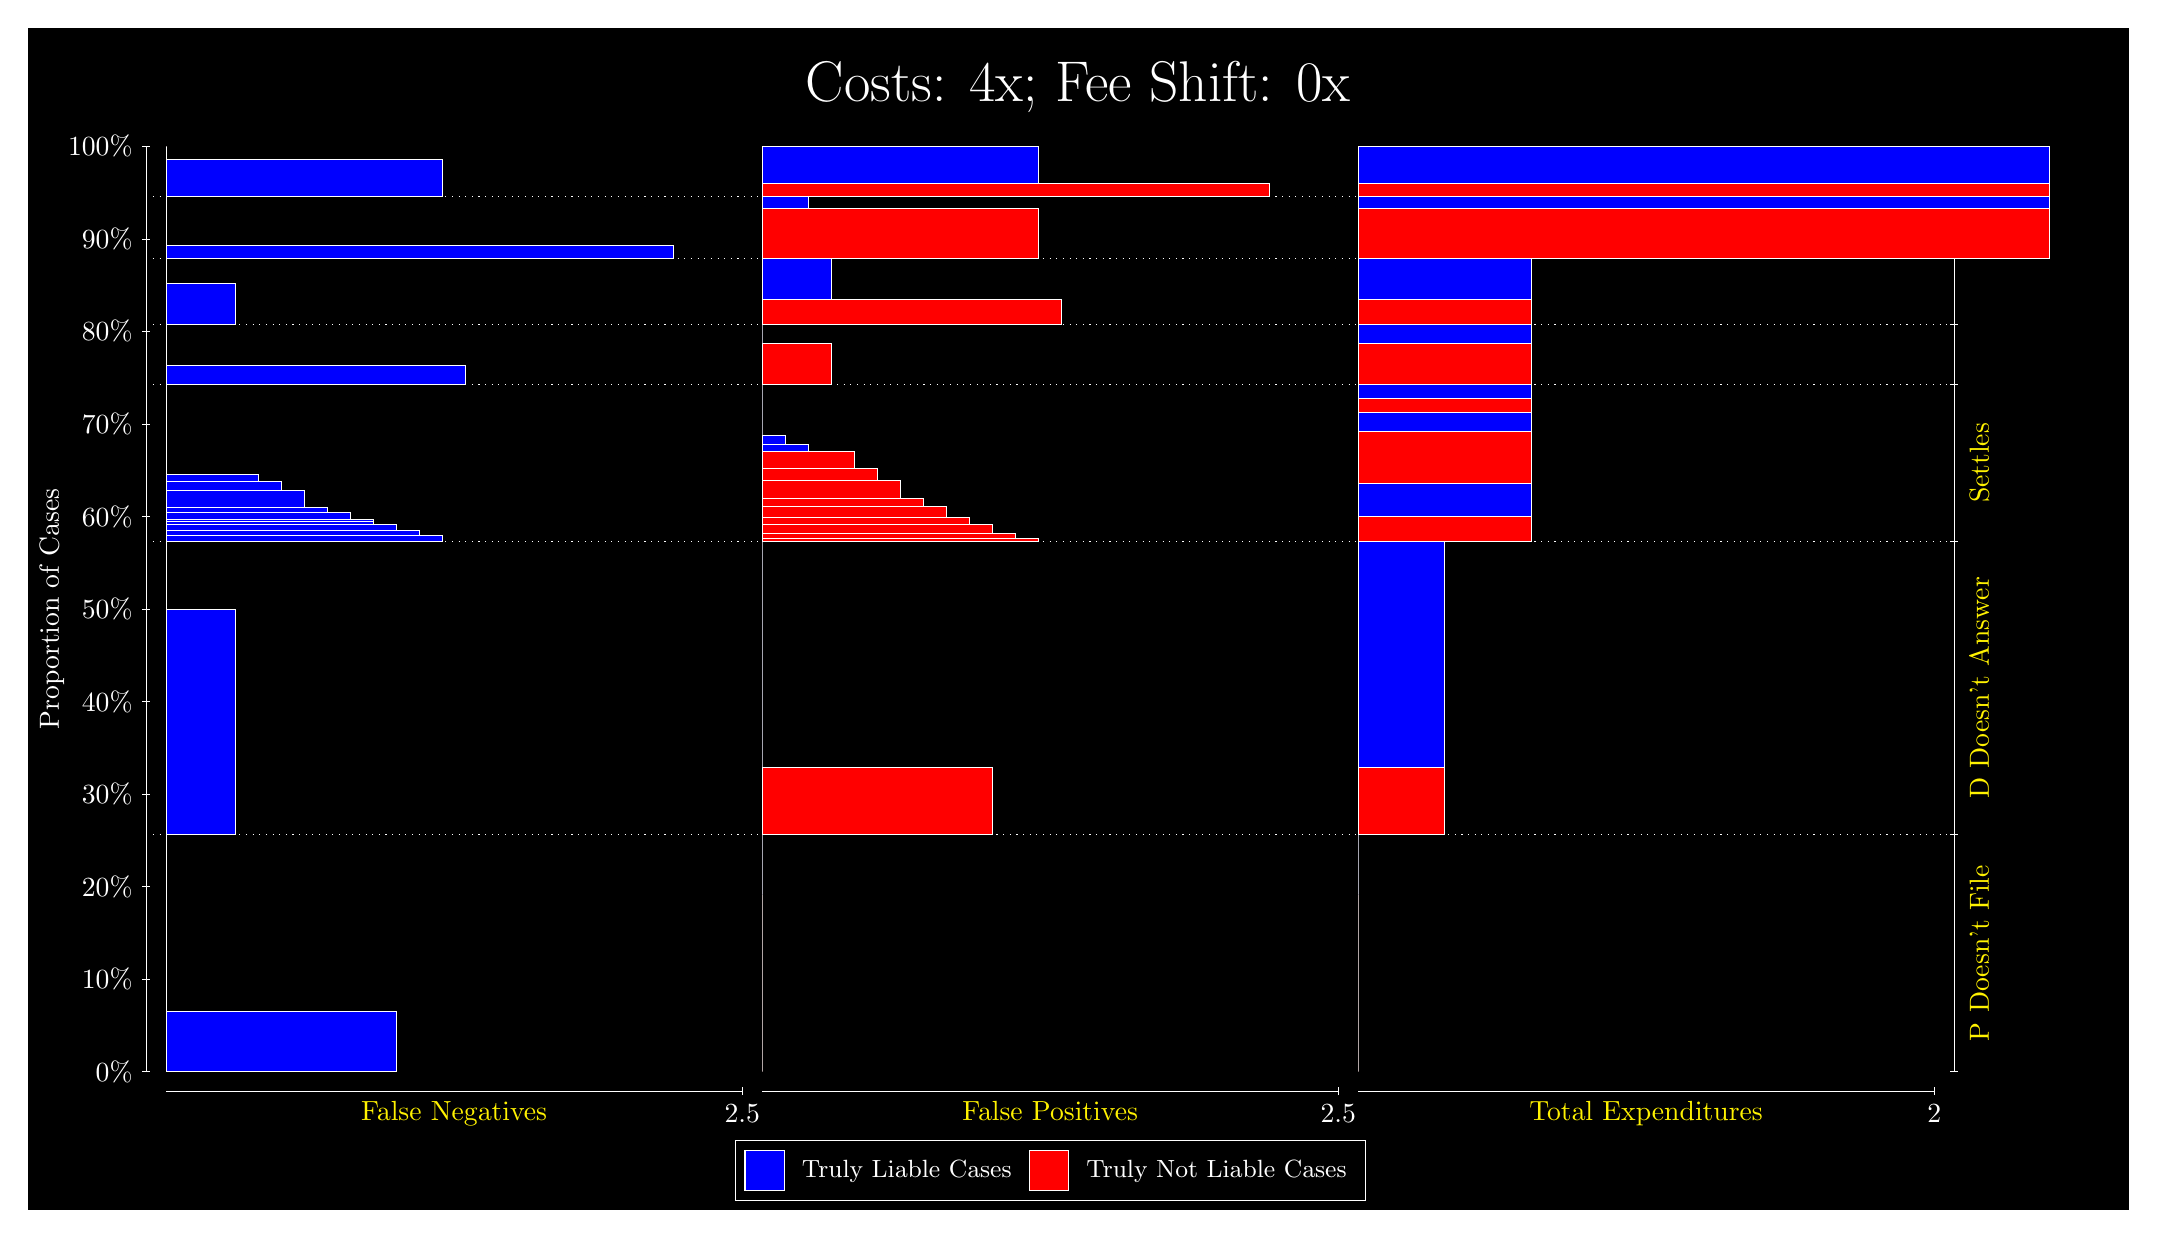
\begin{tikzpicture}
\draw[fill=black] (0,0) rectangle (26.667,15);
\draw[text=white] (0,13.5) rectangle (26.667,15) node[midway] {\huge Costs: 4x; Fee Shift: 0x};
\draw[white, very thin] (1.5,1.75) -- (1.5,13.5);
\node[rotate=90, text=white, anchor=center] at (0.3, 7.625) {Proportion of Cases};
\draw[white, very thin] (1.45,1.75) -- (1.55,1.75);
\node[text=white, anchor=east] at (1.45, 1.75) {0\%};
\draw[white, very thin] (1.45,2.925) -- (1.55,2.925);
\node[text=white, anchor=east] at (1.45, 2.925) {10\%};
\draw[white, very thin] (1.45,4.1) -- (1.55,4.1);
\node[text=white, anchor=east] at (1.45, 4.1) {20\%};
\draw[white, very thin] (1.45,5.275) -- (1.55,5.275);
\node[text=white, anchor=east] at (1.45, 5.275) {30\%};
\draw[white, very thin] (1.45,6.45) -- (1.55,6.45);
\node[text=white, anchor=east] at (1.45, 6.45) {40\%};
\draw[white, very thin] (1.45,7.625) -- (1.55,7.625);
\node[text=white, anchor=east] at (1.45, 7.625) {50\%};
\draw[white, very thin] (1.45,8.8) -- (1.55,8.8);
\node[text=white, anchor=east] at (1.45, 8.8) {60\%};
\draw[white, very thin] (1.45,9.975) -- (1.55,9.975);
\node[text=white, anchor=east] at (1.45, 9.975) {70\%};
\draw[white, very thin] (1.45,11.15) -- (1.55,11.15);
\node[text=white, anchor=east] at (1.45, 11.15) {80\%};
\draw[white, very thin] (1.45,12.325) -- (1.55,12.325);
\node[text=white, anchor=east] at (1.45, 12.325) {90\%};
\draw[white, very thin] (1.45,13.5) -- (1.55,13.5);
\node[text=white, anchor=east] at (1.45, 13.5) {100\%};

\draw[white, very thin] (24.457,1.75) -- (24.457,13.5);
\draw[white, very thin] (24.407,1.75) -- (24.507,1.75);
\node[anchor=west] at (24.407, 1.75) {};
\draw[white, very thin] (24.407,4.758) -- (24.507,4.758);
\node[anchor=west] at (24.407, 4.758) {};
\draw[white, very thin] (24.407,8.4843) -- (24.507,8.4843);
\node[anchor=west] at (24.407, 8.4843) {};
\draw[white, very thin] (24.407,10.477) -- (24.507,10.477);
\node[anchor=west] at (24.407, 10.477) {};
\draw[white, very thin] (24.407,11.238) -- (24.507,11.238);
\node[anchor=west] at (24.407, 11.238) {};
\draw[white, very thin] (24.407,12.076) -- (24.507,12.076);
\node[anchor=west] at (24.407, 12.076) {};
\draw[white, very thin] (24.407,12.868) -- (24.507,12.868);
\node[anchor=west] at (24.407, 12.868) {};
\draw[white, very thin] (24.407,13.5) -- (24.507,13.5);
\node[anchor=west] at (24.407, 13.5) {};

\draw[white, very thin, fill=blue] (1.75,1.75) rectangle (4.6775,2.5117);
\draw[white, very thin, fill=red] (1.75,2.5117) rectangle (1.75,4.758);
\draw[white, very thin, fill=blue] (1.75,4.758) rectangle (2.6283,7.625);
\draw[white, very thin, fill=red] (1.75,7.625) rectangle (1.75,8.4843);
\draw[white, very thin, fill=blue] (1.75,8.4843) rectangle (5.2631,8.5647);
\draw[white, very thin, fill=blue] (1.75,8.5647) rectangle (4.9703,8.6187);
\draw[white, very thin, fill=blue] (1.75,8.6187) rectangle (4.6775,8.6955);
\draw[white, very thin, fill=blue] (1.75,8.6955) rectangle (4.3848,8.7336);
\draw[white, very thin, fill=blue] (1.75,8.7336) rectangle (4.3848,8.7575);
\draw[white, very thin, fill=blue] (1.75,8.7575) rectangle (4.092,8.85);
\draw[white, very thin, fill=blue] (1.75,8.85) rectangle (3.7993,8.9197);
\draw[white, very thin, fill=blue] (1.75,8.9197) rectangle (3.5065,9.1327);
\draw[white, very thin, fill=blue] (1.75,9.1327) rectangle (3.2138,9.2476);
\draw[white, very thin, fill=blue] (1.75,9.2476) rectangle (2.921,9.3311);
\draw[white, very thin, fill=red] (1.75,9.3311) rectangle (1.75,10.477);
\draw[white, very thin, fill=blue] (1.75,10.477) rectangle (5.5558,10.722);
\draw[white, very thin, fill=red] (1.75,10.722) rectangle (1.75,11.238);
\draw[white, very thin, fill=blue] (1.75,11.238) rectangle (2.6283,11.76);
\draw[white, very thin, fill=red] (1.75,11.76) rectangle (1.75,12.076);
\draw[white, very thin, fill=blue] (1.75,12.076) rectangle (8.1906,12.237);
\draw[white, very thin, fill=red] (1.75,12.237) rectangle (1.75,12.868);
\draw[white, very thin, fill=blue] (1.75,12.868) rectangle (5.2631,13.34);
\draw[white, very thin, fill=red] (1.75,13.34) rectangle (1.75,13.5);
\draw[white, very thin, fill=red] (9.3189,1.75) rectangle (9.3189,3.9964);
\draw[white, very thin, fill=blue] (9.3189,3.9964) rectangle (9.3189,4.758);
\draw[white, very thin, fill=red] (9.3189,4.758) rectangle (12.246,5.6173);
\draw[white, very thin, fill=blue] (9.3189,5.6173) rectangle (9.3189,8.4843);
\draw[white, very thin, fill=red] (9.3189,8.4843) rectangle (12.832,8.5199);
\draw[white, very thin, fill=red] (9.3189,8.5199) rectangle (12.539,8.5797);
\draw[white, very thin, fill=red] (9.3189,8.5797) rectangle (12.246,8.7019);
\draw[white, very thin, fill=red] (9.3189,8.7019) rectangle (11.954,8.7911);
\draw[white, very thin, fill=red] (9.3189,8.7911) rectangle (11.661,8.9261);
\draw[white, very thin, fill=red] (9.3189,8.9261) rectangle (11.368,9.0273);
\draw[white, very thin, fill=red] (9.3189,9.0273) rectangle (11.075,9.2612);
\draw[white, very thin, fill=red] (9.3189,9.2612) rectangle (10.783,9.413);
\draw[white, very thin, fill=red] (9.3189,9.413) rectangle (10.49,9.6297);
\draw[white, very thin, fill=blue] (9.3189,9.6297) rectangle (9.9044,9.7132);
\draw[white, very thin, fill=blue] (9.3189,9.7132) rectangle (9.6116,9.8282);
\draw[white, very thin, fill=blue] (9.3189,9.8282) rectangle (9.3189,10.477);
\draw[white, very thin, fill=red] (9.3189,10.477) rectangle (10.197,10.993);
\draw[white, very thin, fill=blue] (9.3189,10.993) rectangle (9.3189,11.238);
\draw[white, very thin, fill=red] (9.3189,11.238) rectangle (13.125,11.554);
\draw[white, very thin, fill=blue] (9.3189,11.554) rectangle (10.197,12.076);
\draw[white, very thin, fill=red] (9.3189,12.076) rectangle (12.832,12.707);
\draw[white, very thin, fill=blue] (9.3189,12.707) rectangle (9.9044,12.868);
\draw[white, very thin, fill=red] (9.3189,12.868) rectangle (15.759,13.028);
\draw[white, very thin, fill=blue] (9.3189,13.028) rectangle (12.832,13.5);
\draw[white, very thin, fill=red] (16.888,1.75) rectangle (16.888,3.9964);
\draw[white, very thin, fill=blue] (16.888,3.9964) rectangle (16.888,4.758);
\draw[white, very thin, fill=red] (16.888,4.758) rectangle (17.986,5.6173);
\draw[white, very thin, fill=blue] (16.888,5.6173) rectangle (17.986,8.4843);
\draw[white, very thin, fill=red] (16.888,8.4843) rectangle (19.083,8.8012);
\draw[white, very thin, fill=blue] (16.888,8.8012) rectangle (19.083,9.2217);
\draw[white, very thin, fill=red] (16.888,9.2217) rectangle (19.083,9.8769);
\draw[white, very thin, fill=blue] (16.888,9.8769) rectangle (19.083,10.126);
\draw[white, very thin, fill=red] (16.888,10.126) rectangle (19.083,10.3);
\draw[white, very thin, fill=blue] (16.888,10.3) rectangle (19.083,10.477);
\draw[white, very thin, fill=red] (16.888,10.477) rectangle (19.083,10.993);
\draw[white, very thin, fill=blue] (16.888,10.993) rectangle (19.083,11.238);
\draw[white, very thin, fill=red] (16.888,11.238) rectangle (19.083,11.554);
\draw[white, very thin, fill=blue] (16.888,11.554) rectangle (19.083,12.076);
\draw[white, very thin, fill=red] (16.888,12.076) rectangle (25.67,12.707);
\draw[white, very thin, fill=blue] (16.888,12.707) rectangle (25.67,12.868);
\draw[white, very thin, fill=red] (16.888,12.868) rectangle (25.67,13.028);
\draw[white, very thin, fill=blue] (16.888,13.028) rectangle (25.67,13.5);
\draw[white, dotted] (1.5,4.758) -- (24.457,4.758);
\draw[white, dotted] (1.5,8.4843) -- (24.457,8.4843);
\draw[white, dotted] (1.5,10.477) -- (24.457,10.477);
\draw[white, dotted] (1.5,11.238) -- (24.457,11.238);
\draw[white, dotted] (1.5,12.076) -- (24.457,12.076);
\draw[white, dotted] (1.5,12.868) -- (24.457,12.868);
\draw[white, very thin] (1.75,1.5) -- (9.0689,1.5);
\node[text=yellow, anchor=north] at (5.4094, 1.5) {False Negatives};
\draw[white, very thin] (9.0689,1.45) -- (9.0689,1.55);
\node[text=white, anchor=north] at (9.0689, 1.45) {2.5};

\draw[white, very thin] (9.3189,1.5) -- (16.638,1.5);
\node[text=yellow, anchor=north] at (12.978, 1.5) {False Positives};
\draw[white, very thin] (16.638,1.45) -- (16.638,1.55);
\node[text=white, anchor=north] at (16.638, 1.45) {2.5};

\draw[white, very thin] (16.888,1.5) -- (24.207,1.5);
\node[text=yellow, anchor=north] at (20.547, 1.5) {Total Expenditures};
\draw[white, very thin] (24.207,1.45) -- (24.207,1.55);
\node[text=white, anchor=north] at (24.207, 1.45) {2};

\node[text=yellow, centered, rotate=90] at (24.777, 3.254) {P Doesn't File};
\node[text=yellow, centered, rotate=90] at (24.777, 6.6212) {D Doesn't Answer};
\node[text=yellow, centered, rotate=90] at (24.777, 9.4804) {Settles};





\draw (12.978300999999998,1.5) node[draw=none] (baseCoordinate) {};
\begin{scope}[align=center]
        \matrix[scale=0.5, draw=white, below=0.5cm of baseCoordinate, nodes={draw}, column sep=0.1cm]{
            \node[rectangle, draw, minimum width=0.5cm, minimum height=0.5cm, fill=blue] {}; &
            \node[draw=none, font=\small, text=white] (B) {Truly Liable Cases}; &
            \node[rectangle, draw, minimum width=0.5cm, minimum height=0.5cm, fill=red] {}; &
            \node[draw=none, font=\small, text=white] (B) {Truly Not Liable Cases}; \\
            };
\end{scope}

\end{tikzpicture}
\end{document}